%% ============================================================
% f2012_sichuan_arts_q19_pyramid.tex
%% 2012 四川卷（文科）第 19 题 三棱锥 P-ABC，∠APB=90°，∠PAB=60°，AB=BC=CA
%% 来源 PDF：普通高考/2012/2012四川文.pdf 第 2 页（印面 774）第 1 栏
%% 坐标取自原页矢量层（bp），原点为图区左上角 (230.0,485.0)，y 向下；虚线照原页。
%% ============================================================
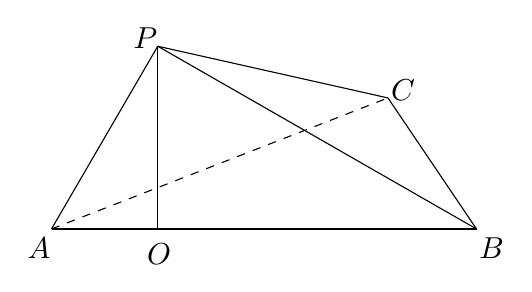
\begin{tikzpicture}[x=1bp,y=-1bp,
  every node/.style={inner sep=0,font=\fontsize{10.5pt}{12.6pt}\selectfont},
  line cap=butt, line join=miter]
  \draw[line width=0.3985bp] (8.547,71.941) -- (161.559,71.941);
  \draw[line width=0.3985bp] (161.559,71.941) -- (129.68,24.762);
  \draw[line width=0.3985bp] (129.68,24.762) -- (46.801,6.145);
  \draw[line width=0.3985bp] (46.801,6.145) -- (8.547,71.941);
  \draw[line width=0.3985bp] (46.801,6.145) -- (161.559,71.941);
  \draw[line width=0.3985bp] (46.801,6.145) -- (46.801,71.941);
  \draw[line width=0.3985bp, dash pattern=on 2.989bp off 2.989bp] (8.547,71.941) -- (129.68,24.762);
  \node[anchor=base west] at (37.87,6.92) {$P$};
  \node[anchor=base west] at (130.62,25.54) {$C$};
  \node[anchor=base west] at (-0.23,82.6) {$A$};
  \node[anchor=base west] at (162.39,82.6) {$B$};
  \node[anchor=base west] at (42.75,84.64) {$O$};
\end{tikzpicture}
